\section{Design of \mytool}
\label{sec:design}

\mytool is designed to resolve the \emph{source identity resolution} bottleneck in \arkts privacy analysis and to produce provenance-annotated evidence subgraphs for auditing. The design is intentionally layered. ArkAnalyzer provides the \arkts IR, project Scene, and call-graph substrate~\cite{arkanalyzer}; HapFlow provides IFDS-based taint propagation over \openharmony programs~\cite{hapflow}. \mytool contributes the missing domain layer: package- and receiver-aware API identity resolution, bounded asynchronous carrier/context recovery, and evidence-preserving subgraph assembly with provenance tracking.

\subsection{Problem Definition and Notation}
\label{subsec:problem_def}

Let a project be $P=\langle F,M,I,E_c\rangle$, where $F$ is the set of \arkts source files, $M$ is the set of methods in ArkAnalyzer IR, $I$ is the set of import bindings, and $E_c \subseteq M\times M$ is the initial call graph. \mytool deliberately separates detector rules $R_D$ from IFDS query rules $R_T$. A detector rule is

\begin{equation}
r_D=\langle pkg,ns,mem,direct,factory,perm,cat\rangle,
\end{equation}

where $pkg$ and $ns$ identify the declaring package and namespace, $mem$ is a method or property token, $direct\in\{true,false,null\}$ distinguishes namespace calls, receiver calls, and property reads, $factory$ is an optional set of receiver-producing methods, $perm$ is permission evidence, and $cat$ is a privacy category. An IFDS query rule is

\begin{equation}
r_T=\langle sig,meta,carrier,i_{cb},i_{src},kind\rangle,
\end{equation}

where $sig$ is an SDK method signature; $meta=\langle module,ns,class,mem,params,lit\rangle$ retains the source identity needed when the frontend cannot resolve that signature; and $carrier\in\{\mathit{return},\mathit{arg},\mathit{callback}\}$ identifies the program value to seed. The source kind distinguishes typed privacy data from explicit framework inputs:
\begin{equation}
kind\in\{\mathit{privacy\_data},\mathit{framework\_input}\}.
\end{equation}
The optional $lit$ component records a string-dispatched event name. For callback sources, $i_{cb}$ is the callback-argument position and $i_{src}$ is the sensitive callback-parameter position. A privacy-data return requires a non-\texttt{void} return type; a callback source requires a typed \texttt{Callback<T>} parameter and a valid carrier index; an argument source is accepted only as an explicitly modeled framework input. Rules without this carrier contract are rejected at load time. Keeping $R_D$ and $R_T$ explicit is essential: a permission-bearing API operation may belong to $R_D$ without producing privacy data, and is therefore not automatically promoted into $R_T$.

\textbf{API identity resolution.} The first task is to compute a semantic identity for each candidate API usage. We define:

\begin{equation}
\mathit{Id}(v) = \langle \mathit{Pkg},\; \mathit{Ns},\; \mathit{Recv},\; \mathit{Mem},\; \mathit{Acc}\rangle,
\end{equation}

where $\mathit{Pkg}$ and $\mathit{Ns}$ are resolved through a namespace-constrained migration map, $\mathit{Recv}$ traces the receiver object back to its source via bounded backward data-flow (e.g., \texttt{cameraMgr} $\leftarrow$ \texttt{getCameraMgr(ctx)}), $\mathit{Mem}$ is the method or property name, and $\mathit{Acc}\in\{\mathit{direct},\mathit{assign},\mathit{indirect},\mathit{property}\}$ classifies the access pattern. Resolution also returns a witness

\begin{equation}
w\in\{\mathit{Namespace},\mathit{IRAlias},\mathit{ExactType},
\mathit{CallTarget},\mathit{FactoryOrigin},\mathit{PropertyRead}\}.
\end{equation}

A usage $u$ is recognized when:

\begin{equation}
\exists s\in Stmt(P),\;\exists r_D\in R_D:\;
\mathit{Accept}(s,r_D,I,A,w),
\end{equation}

where $A$ is the alias relation recovered from imports, assignments, and IR-lowered namespace-member expressions. The recognized usage set is $U_D=\{u \mid \exists s,r_D,w:\mathit{Accept}(s,r_D,I,A,w)\}$.

\textbf{Source carriers and seeds.} For a statement $s$ matching $r_T$, the initial taint fact is determined by the carrier rather than by the API name alone:

\begin{equation}
\mathit{Seed}(s,r_T)=
\begin{cases}
\mathit{lhs}(s), & carrier=\mathit{return},\\
\mathit{arg}_{i_{src}}(s), & carrier=\mathit{arg},\\
\mathit{param}_{i_{src}}(\mathit{ResolveCb}(\mathit{arg}_{i_{cb}}(s))),
    & carrier=\mathit{callback}.
\end{cases}
\end{equation}

Property occurrences in $U_D$ taint the right-hand-side value for detector-local tracing, but enter IFDS only when a corresponding well-formed $R_T$ rule exists. Framework-provided \texttt{Want} values are query sources of kind \textit{framework\_input}, not privacy-API detector occurrences. These distinctions prevent detector coverage, privacy-data seeding, and framework-input analysis from being silently equated.

\textbf{Asynchronous carrier recovery.} The second task is to bind a configured asynchronous source to its consumer. We define:

\begin{equation}
\mathit{SrcBind}(call, cb, param),
\end{equation}

where $call$ is the source API invoke statement, $cb$ is the resolved callback method or Promise handler, and $param$ is the specific parameter through which sensitive data flows. The implementation distinguishes native IFDS propagation from bounded post-IFDS carrier recovery and from callback edges used only for call-chain context; provenance records that distinction.

\textbf{Provenance-annotated subgraph.} The third task is to construct, for each $u\in U_D$, an information-flow subgraph:

\begin{equation}
G_u = \langle V_u,E_u,\lambda_u,\omega_u\rangle,
\end{equation}

where $V_u$ contains API, caller, sink, and taint-fact nodes; $E_u$ contains call, data-flow, and evidence edges, each annotated with a \emph{provenance} label:

\begin{equation}
\omega(e) \in \{\mathit{CG},\;\mathit{Callback},\;\mathit{Lifecycle},\;\mathit{IFDS},\;\mathit{Heuristic}\},
\end{equation}

indicating whether the edge was derived from call-graph resolution, callback analysis, lifecycle model, IFDS propagation, or heuristic association. The provenance label is a derivation record, not a calibrated confidence: IFDS-derived edges depend on CG precision, and a CG edge from a static call may be more reliable than a lifecycle edge from over-approximate transition modeling. Auditors should interpret the label as evidence provenance rather than a global reliability ranking.

\subsection{Architecture Overview}

\begin{figure}[t]
\centering
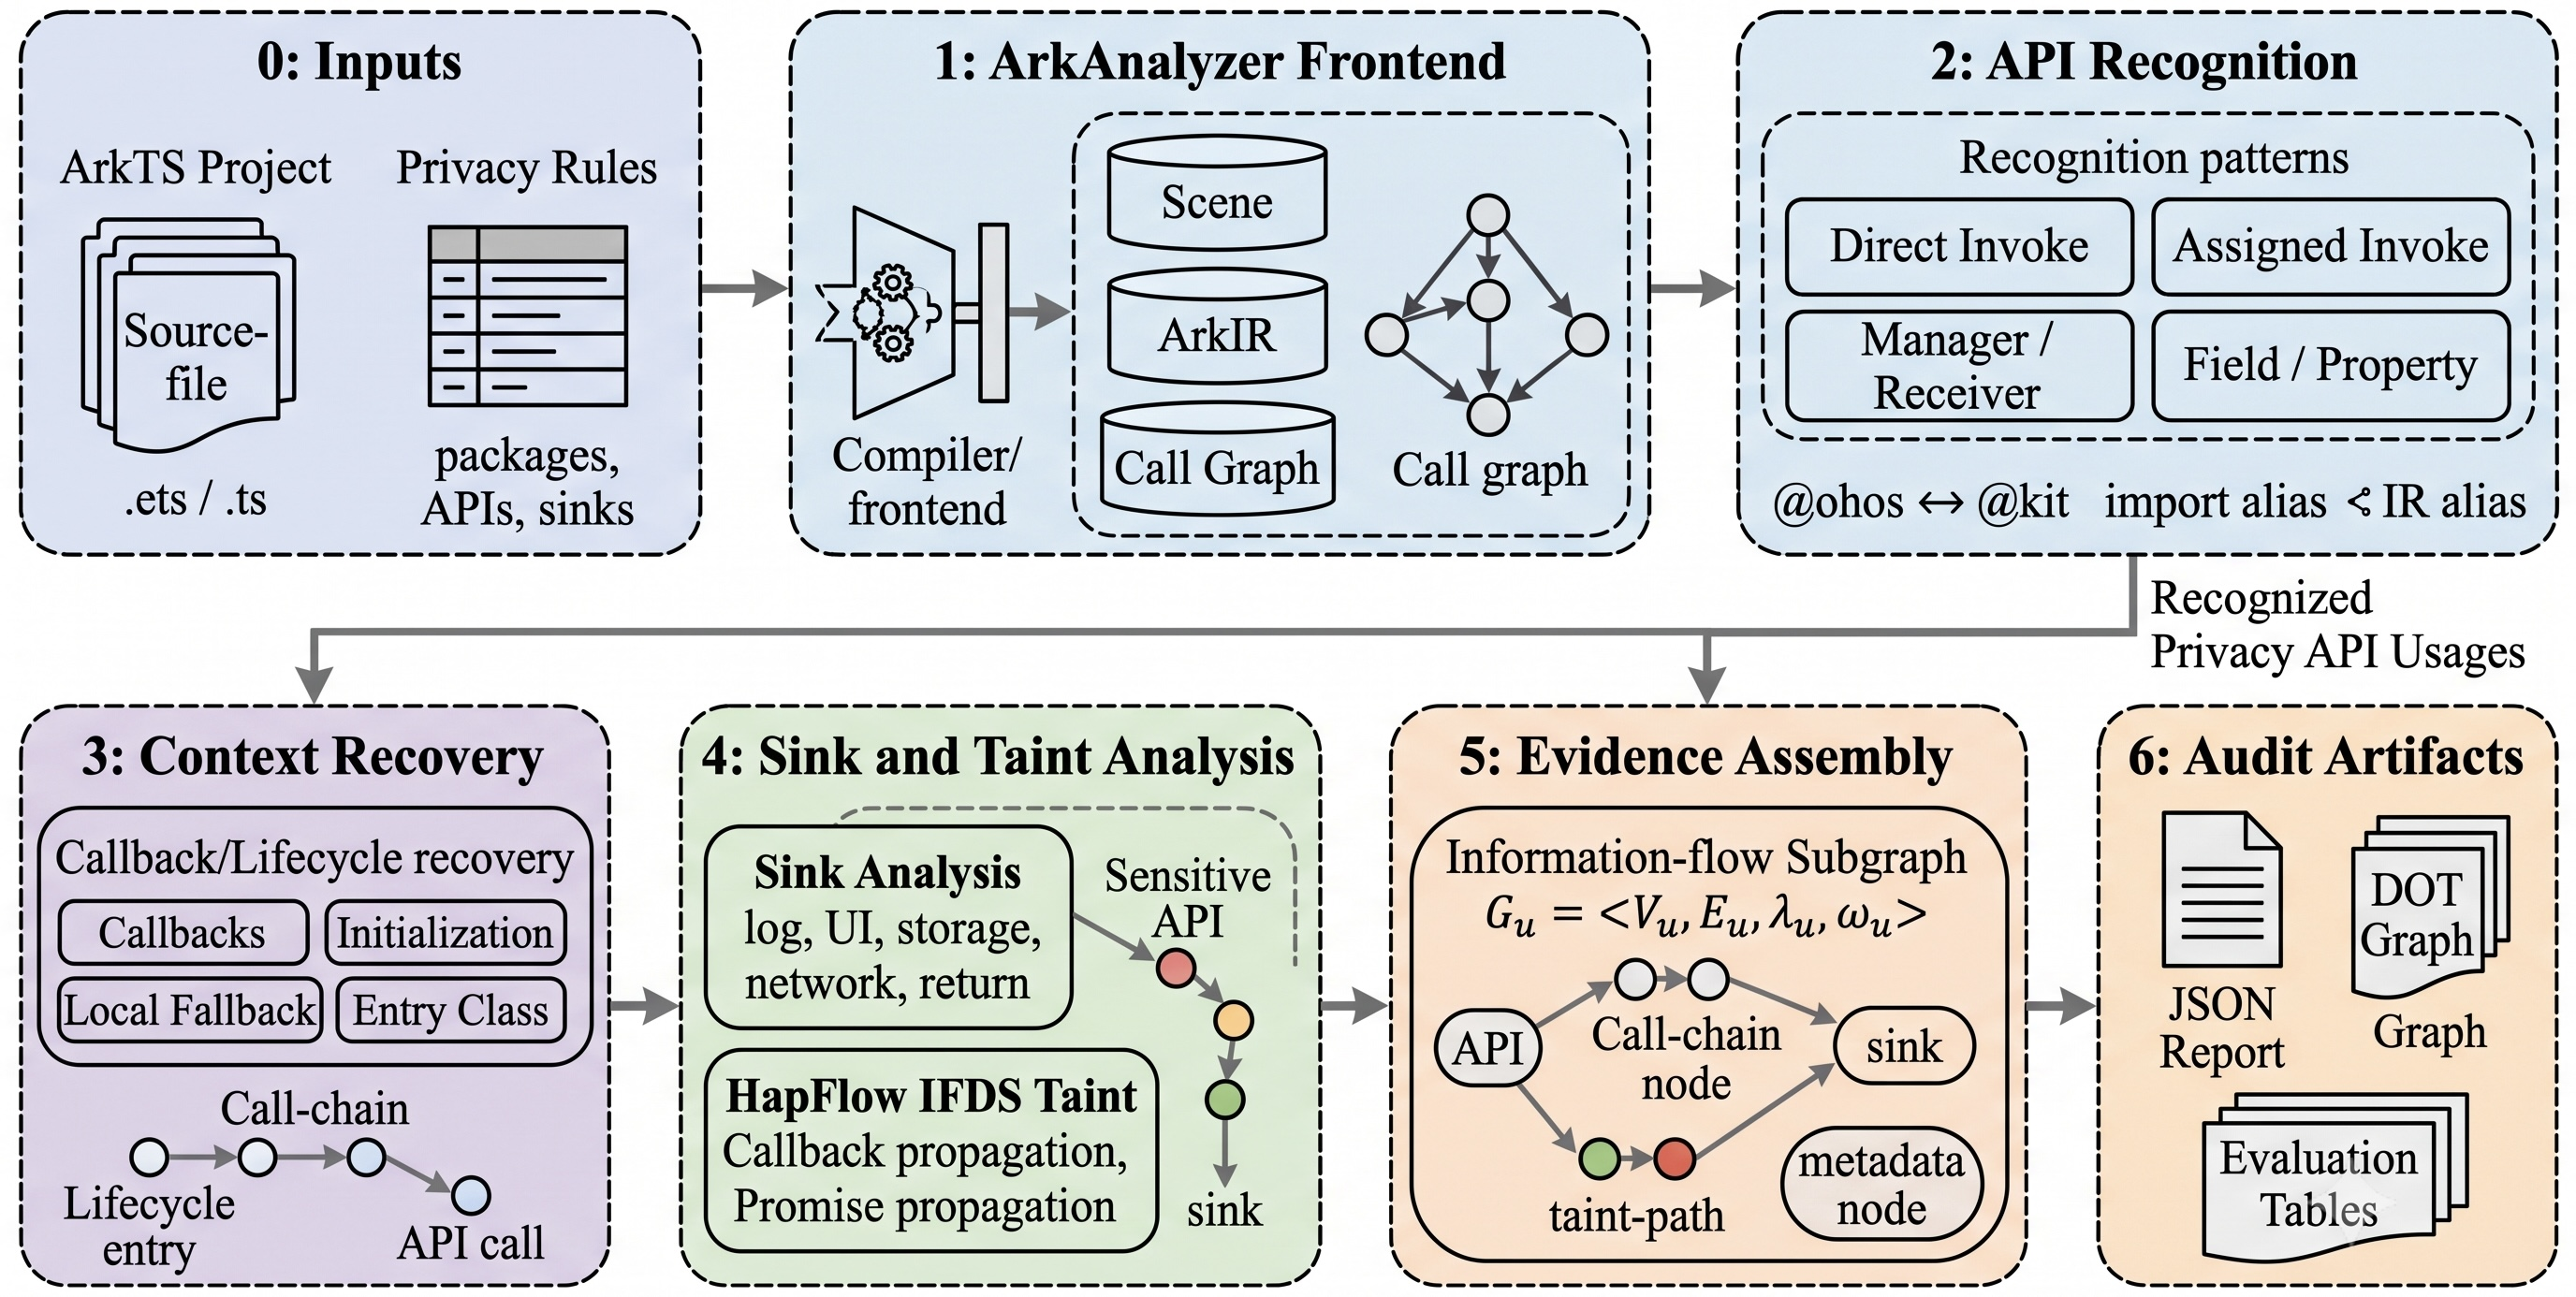
\includegraphics[width=\columnwidth]{figs/arkprism_architecture_generated.jpg}
\caption{\mytool analysis pipeline and evidence assembly.}
\Description{A pipeline diagram showing ArkTS projects and privacy rules flowing through ArkAnalyzer, API recognition, context recovery, sink and taint analysis, evidence assembly, and final audit artifacts.}
\label{fig:architecture}
\end{figure}

Figure~\ref{fig:architecture} gives the end-to-end architecture. Project and rule inputs enter ArkAnalyzer for Scene, IR, and call-graph construction. \mytool then adds three core analyses: (1)~API identity resolution computing $\mathit{Id}(v)$, (2)~bounded asynchronous carrier/context recovery computing $\mathit{SrcBind}(call,cb,param)$ where evidence permits, and (3)~provenance-annotated subgraph assembly with $\omega(e)$ labels. Supporting mechanisms (lifecycle modeling and optional context-sensitive CG) enrich the analysis but are not the primary contributions.

\subsection{Running Example: Why Direct Calls Are Insufficient}
\label{subsec:running_example}

Figure~\ref{fig:running_design} shows an anonymized pattern distilled from manually reviewed benchmark projects. The example is intentionally small, but each highlighted source position corresponds to a real source-level evidence class seen during manual annotation: a manager object returned by a Harmony API, a member call on that manager, a compound namespace API that may be lowered through a temporary, and a local sink that helps an auditor inspect the behavior.

\begin{figure}[t]
\centering
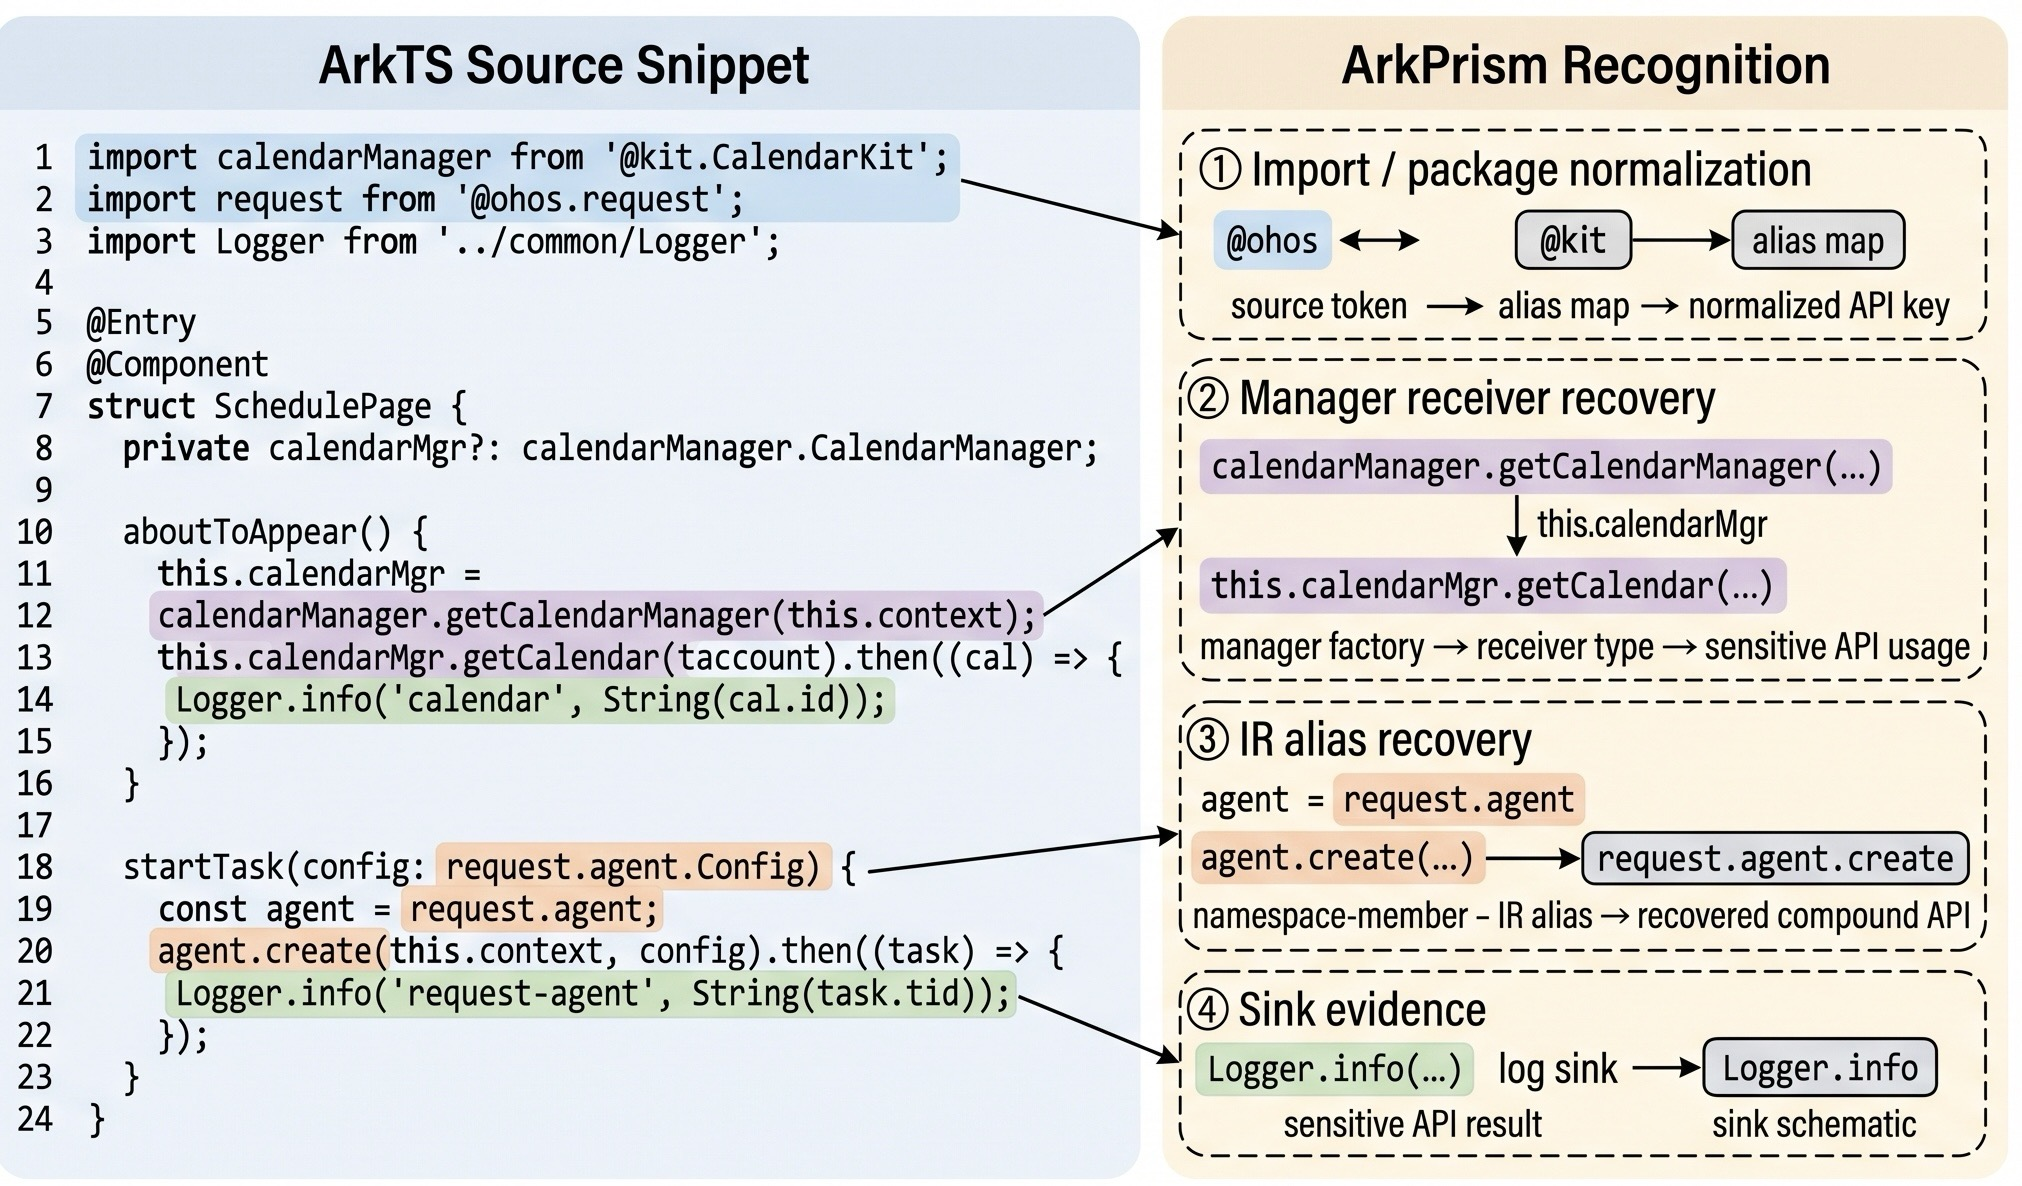
\includegraphics[width=\columnwidth]{figs/2.jpg}
\caption{Running example of API recognition and evidence construction.}
\Description{A three-panel example showing an ArkTS source snippet, ArkPrism recognition steps for import normalization, manager receiver recovery, IR alias recovery, and sink evidence, and the resulting evidence subgraph.}
\label{fig:running_design}
\end{figure}

A direct-call baseline that only matches \texttt{namespace.method(...)} statements can recover neither \texttt{this.calendarMgr.getCalendar(...)} nor \texttt{agent.create(...)} reliably. The former is a member call whose receiver obtains its privacy meaning from \texttt{calendarManager.getCalendarManager}; the latter is a compound namespace API whose \texttt{request.agent} prefix may be assigned to an IR temporary before \texttt{create} is invoked. \mytool therefore treats API recognition as a rule- and evidence-matching problem over imports, aliases, receiver origins, and IR-lowered expressions. The resulting subgraph links the recognized API node to its lifecycle entry \texttt{aboutToAppear}, local sink evidence, optional taint path, and source snippet, rather than returning a flat method-name hit.

\subsection{Namespace-constrained Package Migration}
\label{subsec:pkg_norm}

OpenHarmony API evolution makes exact package matching brittle, but consolidated kit packages are not globally equivalent to their historical modules. We therefore define a directional migration relation over package--namespace pairs,
$\mathcal{M}\subseteq(Pkg\times Ns)\times(Pkg\times Ns)$. For example, the \texttt{deviceInfo} export maps from \texttt{@ohos.deviceInfo} to \texttt{@kit.BasicServicesKit}, while unrelated exports in the same kit do not become compatible. A detector rule $r_D$ and import binding $i$ are compatible when:

\begin{equation}
Compat(i,r_D) \triangleq
(i.pkg,i.ns)=(r_D.pkg,r_D.ns)
\lor ((i.pkg,i.ns),(r_D.pkg,r_D.ns))\in\mathcal{M}.
\end{equation}

The analyzer also derives namespace aliases from import declarations. If a source file contains \texttt{import wifi from '@ohos.wifiManager'}, then $(wifi,\texttt{wifiManager})\in A_{import}$. If it imports a kit package with a default binding, \mytool records both the textual alias and the canonical namespace. Matching therefore uses a normalized API key:

\begin{equation}
key(u)=\langle \mu(pkg_u,ns_u), \sigma(mem_u)\rangle,
\end{equation}

where $\mu$ applies the migration/export map and import-alias normalization to a package--namespace pair, and $\sigma$ normalizes method/property spelling. Evaluation can then report both $key(u)$ and the stricter raw package signature.

\subsection{Package- and Receiver-aware API Identity Resolution}
\label{subsec:identity_resolution}

HapFlow's released namespace--method loader resolves configured entries to SDK declarations. It handles directly resolvable methods, but does not encode executable property reads or retain factory-origin evidence for manager/helper receivers. These are limitations of the released loader and schema, not an impossibility result for all method-signature analyses. \mytool addresses them by computing a semantic identity and an acceptance witness for each candidate usage.

\subsubsection{Identity Function}

Given a candidate statement $s$, \mytool computes $\mathit{Id}(s)$ as defined in Section~\ref{subsec:problem_def}. The key components are $\mathit{Recv}(s)$ (receiver-origin tracing, detailed below) and $\mathit{Acc}(s)$ (access-kind classification).

The candidate predicate is:

\begin{align}
Match(s,r_D,I,A) ={} & Compat(I_s,r_D) \nonumber\\
& \wedge\; \mathit{Id}(s).\mathit{Mem} {=} r_D.mem.
\end{align}

Package compatibility only generates candidates. Acceptance additionally requires access-specific evidence:

\begin{align}
\mathit{Accept}(s,r_D,I,A,w) \triangleq{}&
\mathit{Match}(s,r_D,I,A)\nonumber\\
&{}\land \mathit{Sufficient}(\mathit{Acc}(s),w,r_D),
\end{align}
\begin{equation}
\mathcal{W}_{ind}=\{\mathit{ExactType},\mathit{CallTarget},
\mathit{FactoryOrigin},\mathit{Namespace}\}.
\end{equation}
\begin{equation}
\mathit{Sufficient}(a,w,r_D)=
\begin{cases}
w\in\{\mathit{Namespace},\mathit{IRAlias}\}, & a\in\{\mathit{direct},\mathit{assign}\},\\
w=\mathit{PropertyRead}, & a=\mathit{property},\\
w\in\mathcal{W}_{ind}, & a=\mathit{indirect}.
\end{cases}
\end{equation}

For indirect calls, $\mathit{Namespace}$ means an exact namespace receiver, not merely package presence. It is disabled for generic members such as \texttt{get}, \texttt{on}, \texttt{start}, \texttt{request}, and \texttt{close}; these require type, target, or factory-origin evidence. Property acceptance requires both a property rule ($r_D.direct=null$) and an executable IR field read. Thus, package import or final-token agreement alone is never sufficient.

\paragraph{IFDS source-rule acceptance.}
The IFDS query uses SDK method signatures whenever ArkAnalyzer resolves a call target. For a call whose signature remains unknown after frontend recovery, matching falls back to the configured rule metadata rather than to method name alone. Let $\mathit{Meta}(r_T)$ retain the rule's module, namespace, declaring class, member, arity, parameter types, and any string-dispatched event literal. We define:
\begin{align}
\mathit{Exact}_T(s,r_T) \triangleq{}&
  \mathit{TargetSig}(s)=\mathit{Sig}(r_T),\\
\mathit{Fuzzy}_T(s,r_T) \triangleq{}&
  \mathit{UnknownSig}(s)\land
  \mathit{Mem}(s)=r_T.mem \nonumber\\
  &{}\land \mathit{ArityCompat}(s,r_T)
  \land \mathit{ParamCompat}(s,r_T).
\end{align}
The guard for a generic member and the guard for a string-dispatched overload are:
\begin{align}
\mathit{IdentityGuard}(s,r_T) \triangleq{}&
  \neg\mathit{Generic}(r_T.mem) \nonumber\\
  &{}\lor \mathit{ReceiverOrModuleWitness}(s,\mathit{Meta}(r_T)),\\
\mathit{LiteralGuard}(s,r_T) \triangleq{}&
  \neg\mathit{HasEventLiteral}(r_T)\nonumber\\
  &{}\lor \mathit{ArgLiteral}(s,0)=\mathit{EventLiteral}(r_T).
\end{align}
The source call is accepted iff
\begin{equation}
\mathit{Accept}_T(s,r_T)\triangleq
\mathit{Exact}_T(s,r_T)\lor
\bigl(\mathit{Fuzzy}_T(s,r_T)\land
\mathit{IdentityGuard}(s,r_T)\land
\mathit{LiteralGuard}(s,r_T)\bigr).
\end{equation}
Consequently, an unresolved call such as \texttt{avPlayer.on('error',...)} cannot match a configured geolocation or sensor event merely because both use \texttt{on} with the same arity. This predicate governs IFDS source seeding and is separate from the detector acceptance predicate above.

\subsubsection{Receiver-Origin Tracing}

The key addition beyond the released namespace--method loader is $\mathit{Recv}(s)$. For a statement $s: x.m(\ldots)$ where $x$ is a local or field variable, \mytool traces $x$ backward through assignments and instance-invoke bases to find its origin, subject to a tracing bound of $k_{recv}$ steps (default 8) to avoid unbounded backward exploration:

\begin{equation}
\mathit{Recv}(s) \!=\!
\begin{cases}
\mathit{Ns}(def), & x {\leftarrow} invoke(q.f()),\;f{\in}R,\\
\mathit{Recv}(def), & x {\leftarrow} y,\;y\text{ has known origin},\\
\mathit{TF}(x), & \mathit{type}(x){=}T,\;T{\in}\mathit{SDK},\\
\bot, & \text{unresolvable in }k_{recv}\text{ steps.}
\end{cases}
\end{equation}

The first case covers the common pattern $mgr \leftarrow getManager(ctx);\; mgr.getData(cb)$, where the receiver $mgr$ originates from a privacy API factory call. The second case propagates origin through intra-procedural assignment chains and instance-invoke bases. The third case ($\mathit{TF}$) uses an exactly compatible declared SDK type. Inter-method field assignments are not claimed as origin-proven unless the defining statement or an exact type/target identity is recovered; otherwise the call is rejected. This rule avoids silently treating package import plus method-name agreement as a typed call target.

\subsubsection{Access-Kind Classification}

Each recognized usage receives an $\mathit{Acc}$ label:
\begin{itemize}
    \item $\mathit{direct}$: bare invoke statement, e.g., \texttt{id.getOAID(cb)};
    \item $\mathit{assign}$: invoke with return value assigned, e.g., \texttt{net = getDefaultNet()};
    \item $\mathit{indirect}$: invoke on a traced receiver, e.g., \texttt{mgr.getData(cb)} where $\mathit{Recv}(mgr)\neq\bot$;
    \item $\mathit{property}$: field/property read, e.g., \texttt{deviceInfo.productModel}.
\end{itemize}

Table~\ref{tab:identity_examples} illustrates how $\mathit{Id}$ resolves each access kind.

\begin{table}[t]
\centering
\caption{API identity resolution examples.}
\label{tab:identity_examples}
\small
\begin{tabularx}{\columnwidth}{@{}lYl@{}}
\toprule
Source pattern & $\mathit{Id}(s)$ & $\mathit{Acc}$ \\
\midrule
\texttt{id.getOAID(cb)} & $\langle$BasicSvc, id, $\bot$, getOAID, $\mathit{direct}\rangle$ & direct \\
\texttt{net=getDefaultNet()} & $\langle$NetworkKit, net, $\bot$, getDefaultNet, $\mathit{assign}\rangle$ & assign \\
\texttt{mgr.getData(cb)} & $\langle$BasicSvc, mgr, getMgr, getData, $\mathit{indirect}\rangle$ & indirect \\
\texttt{deviceInfo.brand} & $\langle$BasicSvc, devInfo, $\bot$, brand, $\mathit{property}\rangle$ & property \\
\bottomrule
\end{tabularx}
\end{table}

IR-lowered multi-segment APIs require an additional alias relation $A_{ir}$. For assignments of the form $t := q.member$, \mytool records $(t,q.member)\in A_{ir}$. A later statement \texttt{t.create(...)} is matched as \texttt{q.member.create(...)} if the composed signature appears in $R_D$. This is essential for APIs such as \texttt{request.agent.create}, whose namespace can disappear after lowering.

\subsection{Lifecycle State Machine Model}
\label{subsec:lifecycle}

\openharmony applications follow a structured lifecycle managed by the system runtime. A \texttt{UIAbility} transitions through creation, foreground, background, and destruction phases; custom components follow appearance, build, page visibility, and disappearance phases; UI callbacks are registered during component build and triggered by user interaction. These transitions are \emph{implicit}---the runtime invokes lifecycle methods without visible call edges in application code---so a static analyzer that treats each lifecycle method as an independent entry point misses cross-phase data flow.

\mytool models the \openharmony application lifecycle as a three-layer state machine. Let the lifecycle model be:
\begin{equation}
\mathcal{L} = \langle \Phi_a, \Phi_c, \delta_a, \delta_c, \delta_{cross} \rangle,
\end{equation}
where $\Phi_a$ is the set of ability phases (e.g., \texttt{CREATING}, \texttt{FOREGROUNDED}), $\Phi_c$ the component phases (e.g., \texttt{APPEARING}, \texttt{BUILT}), $\delta_a \subseteq \Phi_a \times \Phi_a$ the ability transition relation, $\delta_c \subseteq \Phi_c \times \Phi_c$ the component transition relation, and $\delta_{cross} \subseteq \Phi_a \times \Phi_c$ the cross-layer transition relation.  Cross-layer transitions capture implicit calls such as \texttt{onForeground} $\to$ \texttt{aboutToAppear}.

The lifecycle modeler discovers ability classes by checking superclass inheritance from \texttt{UIAbility}, \texttt{Ability}, and extension ability base classes; component classes by checking superclass (\texttt{CustomComponent}, \texttt{ViewPU}), decorators (\texttt{@Component}), or the presence of two or more component lifecycle methods; and callback methods by scanning IR statements for \texttt{CommonMethod.*} invocations and extracting \texttt{FunctionType} arguments.

Lifecycle information is consumed in two distinct ways. For call-chain recovery, each transition $(m_i,m_j)\in\delta_a\cup\delta_c\cup\delta_{cross}$ becomes a provenance-labeled implicit edge. For IFDS, the model orders entry methods in a synthetic \texttt{DummyMain}: ability creation and foreground callbacks precede component initialization and UI callbacks, followed by background and destruction phases. The bounded default removes the standard back edge from the final entry to the loop header, preventing arbitrary destruction-to-creation cycles. Repeatable event classes may receive one additional explicit firing, but no unbounded loop. The IFDS solver derives interprocedural targets from the Scene and pointer information; it does not consume the separately augmented report call graph.

\subsection{Asynchronous Carrier and Context Recovery}
\label{subsec:async_binding}

\openharmony privacy APIs often deliver sensitive data through asynchronous callbacks and Promise chains rather than direct return values. For example, \texttt{geoLocationManager.getCurrentLocation(callback)} passes location data to a callback parameter, while \texttt{wifiManager.getLinkedInfo().then(callback)} delivers Wi-Fi state through a Promise resolution. Standard call-to-return propagation does not by itself establish the connection between a source invocation and a callback parameter or Promise resolution, so these constructs require explicit transfer rules.

\mytool formalizes carrier binding as $\mathit{SrcBind}(call, cb, param)$ (Section~\ref{subsec:problem_def}). The five recovery rules do not all modify the same analysis. T1, T4, and T5 add bounded source-to-sink outcomes after the core IFDS run when ArkIR lacks an explicit continuation edge; T2 and T3 add callback edges to the report call graph and therefore improve context recovery rather than seeding IFDS facts. Table~\ref{tab:transfer_rules} makes this execution domain explicit.

\begin{table}[t]
\centering
\caption{Asynchronous carrier and context recovery rules.}
\label{tab:transfer_rules}
\small
\begin{tabularx}{\columnwidth}{@{}lYYll@{}}
\toprule
Rule & Construct & Recovery relation & Output & Domain \\
\midrule
T1 & Callback source & $Resolve(a_i)\!\to\!cb.param_j$ & May-path & Post-IFDS \\
T2 & Field callback & $Read(this.f)\!\to\!cb$ & Call edge & Report CG \\
T3 & Builder option & $Arg(bld,f)\!\to\!cb$ & Call edge & Report CG \\
T4 & Promise \texttt{then} & $ret(src)\!\to\!then_j.param$ & May-path & Post-IFDS \\
T5 & \texttt{async/await} & $resolve_{arg}\!\to\!await_{res}$ & May-path & Post-IFDS \\
\bottomrule
\end{tabularx}
\end{table}

\subsubsection{T1: Callback Parameter Binding}

When an $R_T$ source accepts a callback as a direct argument at position $i$, the binding is $\mathit{SrcBind}(s, cb, param_j)$ where $cb = Resolve(a_i)$ and $param_j$ is the callback parameter selected by the rule's carrier metadata. The post-IFDS phase accepts only typed or definition-backed callbacks. Resolution applies three strategies in order:

\begin{equation}
Resolve(a_i) =
\begin{cases}
m_f, & a_i \in FuncType \land m_f = Lkp(a_i.sig)\\
m_c, & a_i \in ClosureType \land m_c = Lkp(Ext(a_i))\\
m_l, & a_i \in Local \land m_l = Trc(a_i)
\end{cases}
\end{equation}

$FunctionType$ resolution ($Lkp$) extracts the method signature from the compiler-generated function type and looks up the corresponding method in the declaring class. $ClosureType$ resolution ($Ext$+$Lkp$) parses the closure variable name from the closure type string (e.g., \texttt{closures: \_\_lambda1}) and performs a method name lookup. $Local$ variable tracing ($Trc$) follows the definition chain: if $a_i$ is assigned from a \texttt{new LambdaClass()} expression, the ClosureType of the constructor call provides the callback method. Example: \texttt{getData((err,data)$\Rightarrow$...)} resolves the arrow function to its IR method and binds \texttt{data} as the sensitive parameter.

The tracer seeds only $param_j$ selected by $r_T.i_{src}$, not every callback parameter. It propagates through ArkIR value-use edges and assignments, and accepts a sink only when a sink argument structurally depends on the current fact. IR-local names are never compared by substring, and control dependence alone does not constitute an explicit data-flow edge.

\subsubsection{T2: Field-Stored Callback Binding}

ArkUI components frequently store callback functions in class fields (e.g., \texttt{this.handler = () => \{...\}}). The callback is registered with a framework API at a later point, creating a temporal gap between definition and invocation. \mytool reads the field value at the registration site and traces it to the assignment, adding $Read(this.f)\to cb$ to the report call graph. This handles the pattern where \texttt{this.onSelect} is passed to \texttt{List.onSelect(this.onSelect)} in a component's build method. T2 supplies entry/call context; it does not by itself assert a sensitive carrier or inject an IFDS fact.

\subsubsection{T3: Builder-Option Callback Binding}

ArkUI builder APIs accept configuration objects whose fields are callback functions (e.g., \texttt{bindPopup(\{builder: popupBuilder\})}). T3 extracts the callback from a named option field, $Arg(bld,f)\to cb$, and adds the recovered owner--builder edge to the report call graph. The pattern is structurally distinct from T1 because the callback is nested inside a lowered object initializer rather than passed as a positional source callback. As with T2, the edge provides call context and is not an IFDS seed.

\subsubsection{T4: Promise \texttt{.then()} Chain Binding}

Promise \texttt{.then()} chains can carry a source return value through Promise resolution to a callback parameter. When the core IFDS result lacks that continuation, the bounded supplement recognizes three sub-patterns:

\textbf{Direct chaining:} $sourceApi(args).then(cb)$ creates $\mathit{SrcBind}(sourceStmt, cb, param)$ with $Edge(sourceStmt, cb_{param})$.

\textbf{Variable chaining:} $x = sourceApi(args);\; x.then(cb)$ creates $Edge(sourceStmt, x_{assign}) \cup Edge(x_{assign}, cb_{param})$.

\textbf{Sequential chaining:} $x.then(cb_1).then(cb_2)$ creates $\bigcup_{i} Edge(cb_{i-1}, cb_{i})$, propagating taint through the chain.

\subsubsection{T5: \texttt{async/await} Bridge Binding}

An \texttt{async} function that \texttt{await}s a Promise-wrapped source API creates an implicit binding between the resolved value and the local variable:

\begin{multline}
data = await\; promiseMethod() \;\Rightarrow\;\\
Edge(resolve_{arg}, await_{res}) \cup Edge(await_{res}, data_{uses})
\end{multline}

where $resolve_{arg}$ traces from the \texttt{resolve()} call inside the Promise executor to the awaited result. The supplement requires a definition-backed Promise owner and separately labels the resulting path; it does not claim that the core IFDS supergraph contains the implicit executor-to-\texttt{await} edge.

\subsubsection{Algorithm}

Algorithm~\ref{alg:callback} summarizes the post-IFDS portion (T1, T4, and T5). It does not modify IFDS flow functions or the exploded supergraph. Instead, it scans configured sources whose continuation edge is absent, resolves only typed callbacks or definition-backed Promise owners, performs bounded local/interprocedural tracing, and appends separately provenance-labeled outcomes. T2 and T3 are constructed by the callback-augmented report call graph in Section~\ref{subsec:async_binding}; they are intentionally absent from Algorithm~\ref{alg:callback}.

\begin{algorithm}[H]
\caption{Post-IFDS Asynchronous Carrier Recovery}
\label{alg:callback}
\footnotesize
\begin{algorithmic}[1]
\Require Method $m$, IFDS source rules $R_T$, existing outcomes $O$, bounds $B$
\Ensure $\Call{Deduplicate}{O\cup A}$; each $a\in A$ has provenance \textsc{AsyncSupplement}
\State $A \gets \emptyset$
\ForAll{invoke statements $s \in m$}
  \State $src \gets \Call{CallSource}{s,R_T}$
  \If{$src \neq \emptyset \land src.carrier = \mathit{callback}$} \Comment{T1}
    \State $cb \gets \Call{Resolve}{s.args[src.cbIdx]}$
    \If{$cb\neq\emptyset \land src.srcIdx<|cb.params|$}
      \State $p \gets cb.params[src.srcIdx]$
      \State $A \gets A \cup \Call{TraceToSink}{cb,p,\mathit{Path}(s),B}$
    \EndIf
  \EndIf
  \If{$s$ is a \texttt{then} invocation on base $b$} \Comment{T4}
    \If{$b$ is a configured source invocation}
      \State $si \gets b$
    \Else
      \State $si \gets \Call{FindSrcDef}{m,b}$
    \EndIf
    \If{$si \neq \emptyset$}
      \State $cb \gets \Call{Resolve}{s.args[0]}$
      \If{$cb\neq\emptyset$}
        \State $A \gets A \cup \Call{TraceThenToSink}{m,si,cb,B}$
      \EndIf
    \EndIf
  \EndIf
\EndFor
\ForAll{await sites $a \in m$ with promise $p$} \Comment{T5}
  \State $ow \gets \Call{FindPromiseOwner}{p}$
  \If{$ow\neq\emptyset$}
    \State $rf \gets \Call{CollectResolveFacts}{ow}$
    \If{$rf\neq\emptyset$}
      \State $A \gets A \cup \Call{TraceToSink}{m,a.res,\mathit{Path}(rf)\cup\mathit{Path}(a),B}$
    \EndIf
  \EndIf
\EndFor
\State \Return $\Call{Deduplicate}{O\cup A}$
\end{algorithmic}
\end{algorithm}

\subsection{Context-Sensitive Call Graph Construction}
\label{subsec:context_sensitive}

\mytool supports $k$-limited context-sensitive call graph construction using ArkAnalyzer's pointer analysis infrastructure, where $k$ controls the depth of calling context tracked per invocation. At $k=0$ the analysis is context-insensitive; at $k\geq 1$ call sites receive distinct contexts. Context sensitivity is an optional substrate rather than a claimed contribution; the main evaluation fixes the setting for all compared configurations instead of mixing call-graph precision with API-recognition effects.

\subsection{Callback-augmented Call-chain Recovery}

Given a recognized usage $u$ inside method $m_u$, call-chain recovery searches a reverse graph:

\begin{equation}
E_r = (E_c)^{-1} \cup (E_{invoke})^{-1} \cup (E_{cb})^{-1} \cup (E_{init})^{-1}.
\end{equation}

Here $E_c$ is the ArkAnalyzer call graph, $E_{invoke}$ contains IR-level call edges absent from the graph, $E_{cb}$ contains callback edges recovered from FunctionType/ClosureType values, field callback assignments, and builder-option callbacks, and $E_{init}$ links generated initialization methods to their owning class or component context. The recovered chain set is:

\begin{align}
C_u = \{\, &\pi=(m_0,\ldots,m_u) \mid
m_0\in Entry \cup Init \cup Unknown, \nonumber\\
& (m_i,m_{i+1})\in E_r^{-1}\,\}.
\end{align}

Each chain receives an entry-evidence class:

\begin{equation}
\kappa(\pi)=
\begin{cases}
framework, & m_0\in Entry\\
initialization, & m_0\in Init\\
local, & \pi=(m_u) \text{ and no predecessor is found}\\
unknown, & \text{otherwise.}
\end{cases}
\end{equation}

\mytool does not collapse these classes into a single coverage number. A local fallback chain is useful evidence that the API usage exists in a method, but it is not a recovered framework-entry path. This distinction is preserved in the report and in the evaluation tables.

\subsection{Sink and Taint Attachment}

For each detector occurrence $u\in U_D$, local tracing extracts statements $K_D(u)$ that may expose privacy-related data through logging, UI display, storage, network transfer, or data return. Sink resolution requires an exact configured method token and compatible receiver/namespace evidence; in particular, substring agreement such as \texttt{set} versus \texttt{setData} is rejected.

The IFDS query is configured independently by $R_T$ and its sink set $K_T$. Let $S_P$ and $S_F$ be source statements whose rules have kind \textit{privacy\_data} and \textit{framework\_input}, respectively. The solver computes

\begin{equation}
T_I \subseteq S_T \times K_T \times Path,
\end{equation}

where $S_T=S_P\uplus S_F$ is the disjoint typed-source universe resolved from $R_T$. Each tuple $\langle s,k,\rho\rangle$ means that the carrier seeded at $s$ may reach configured sink $k$ along path $\rho$. The bounded post-IFDS rules produce a separate set

Each seeded fact also carries an immutable source witness
\begin{equation}
\epsilon(s)=\langle kind,pkg,ns,cls,mem,carrier,sig,rule\rangle,
\end{equation}
where $kind\in\{\mathit{privacy\_data},\mathit{framework\_input}\}$ and the remaining fields identify the resolved API, carrier position, SDK signature, and rule provenance. Normal, call, and return transfers copy $\epsilon(s)$ unchanged; fact and edge identities include it. Consequently, two values reaching the same statement from different configured sources remain distinct, and the report obtains its source endpoint from $\epsilon(s)$ rather than inferring it from the first statement in $\rho$.

\begin{equation}
T_A \subseteq S_T \times K_T \times Path,
\end{equation}

and the report exposes $T_Q=T_I\cup T_A$, stratified as
\begin{equation}
T_P=\{q\in T_Q\mid src(q)\in S_P\},\qquad
T_F=\{q\in T_Q\mid src(q)\in S_F\}.
\end{equation}
For duplicate endpoint/path outcomes, path provenance is retained as

\begin{equation}
\tau(q)\in\{\mathit{ifds},\mathit{async\_supplement},\mathit{both}\}.
\end{equation}

A partial linkage relation

\begin{equation}
L\subseteq U_D\times T_P
\end{equation}

is created only when project, normalized source location, and compatible API identity agree. Framework-input paths are never linked to privacy-API detector occurrences. Linked privacy-data paths are attached to the corresponding $G_u$; unlinked configured-query paths remain project-level taint evidence rather than being forced onto a detector occurrence. Consequently, detector-local sink-positive projects and configured-query-path-positive projects are not set-inclusion counts. The corpus evaluation reports both evidence universes and both source kinds separately.

\subsubsection{Provenance Annotation}

Each edge $e \in E_u$ carries a provenance label $\omega(e) \in \{\mathit{IFDS},\;\mathit{Callback},\;\mathit{Lifecycle},\;\mathit{CG},\;\mathit{Heuristic}\}$ (Section~\ref{subsec:problem_def}), recording \emph{how} the edge was derived: $\mathit{IFDS}$ for solver-propagated facts; $\mathit{Callback}$ for a report-CG callback edge or post-IFDS asynchronous supplement; $\mathit{Lifecycle}$ for implicit phase transitions; $\mathit{CG}$ for call-graph edges; and $\mathit{Heuristic}$ for name-based inferences without formal proof. The record also identifies its producing phase, so a callback supplement is not mislabeled as an IFDS proof. Provenance is not a calibrated confidence score: an IFDS edge depends on call-graph precision, and a lifecycle edge may over-approximate feasible order. We therefore evaluate flow classification separately from evidence availability and do not convert provenance labels into an unsupported probability of correctness.

\subsection{Analysis Contract and Soundness Envelope}
\label{subsec:analysis_contract}

\mytool is a soundy audit analysis, not a proof system. Its recognition claim is relative to (i) ArkAnalyzer successfully lowering a source construct to IR, (ii) the API appearing in the fixed rule set, and (iii) package compatibility plus the required namespace, receiver, origin, or target-signature evidence satisfying $\mathit{Accept}$. Native code, dynamic loading, reflection-like runtime dispatch, and APIs absent from the rule set lie outside this contract. A recognized API is evidence of use, not evidence of a privacy violation.

IFDS and asynchronous-supplement results are may-flows under their respective source/sink and reachability models. The report preserves their producer and does not convert a detector occurrence into an IFDS source without a source-endpoint link. Every run records one of three solver states: complete, resource-bounded, or failed. Resource-bounded and failed cases are never reclassified as zero-flow applications. Edge deduplication is scoped by IR statement, value identity, access path, and source witness; textual equality alone is insufficient because same-named locals in different methods and facts from different seeds are distinct. These requirements are regression-tested on HapBench positive and negative cases and are also enforced by the isolated-process corpus runner.

\subsection{Corpus-scale Hardening}

Corpus-scale execution requires additional engineering. SDK files are loaded lazily into the Scene only when taint analysis starts, avoiding SDK-induced type instability during initial project construction. Source and sink JSON rules expand SDK-path placeholders at runtime. IFDS budgets are explicit. Each project runs in a fresh process because retaining SDK-augmented scenes across projects causes cumulative heap growth; per-project logs and status files make timeouts and failures visible. If pointer analysis fails, the runner records the warning and continues only with evidence whose producing phase completed. These choices prevent incomplete analysis states from silently becoming negative results.

The complete pipeline follows a fixed order: Scene construction, lifecycle modeling, report call-graph construction, import/alias extraction, API identity resolution via $\mathit{Accept}$, callback-augmented chain recovery, detector-local sink tracing, IFDS taint analysis from the lifecycle-aware \texttt{DummyMain}, bounded asynchronous supplementation, endpoint linkage, and subgraph assembly. A key property is that \mytool never treats a missing layer as proof of absence: if a call-chain predecessor is absent, the usage still becomes a local evidence chain; if a taint path has no compatible detector endpoint, both records remain visible but unlinked.
